\documentclass[
  accentcolor=tud1c,	% Color theme for TUD corporate design
  colorbacktitle,		% Titlepage has colored background for title area
  inverttitle,			% Font color of title on titlepage is inverted
  german,
  twoside
]{tudexercise}

\usepackage[ngerman]{babel}
\usepackage{units}
\usepackage{hyperref}
\usepackage{booktabs}
\usepackage[utf8]{inputenc}
\usepackage{algorithm2e}
\usepackage{paralist}

\definecolor{commentgreen}{RGB}{50,127,50}


\usepackage{listings}
\lstloadlanguages{C++,[gnu]make}
\lstset{language=C++}
\lstset{captionpos=b}
\lstset{tabsize=3}
\lstset{breaklines=true}
\lstset{basicstyle=\ttfamily}
\lstset{columns=flexible,keywordstyle=\color{purple},stringstyle=\color{blue},commentstyle=\color{commentgreen}}
\lstset{literate=%
	{Ö}{{\"O}}1
	{Ä}{{\"A}}1
	{Ü}{{\"U}}1
	{ß}{{\ss}}2
	{ü}{{\"u}}1
	{ä}{{\"a}}1
	{ö}{{\"o}}1
	{'}{{\textquotesingle}}1
}

\lstnewenvironment{lstmake} %
{\lstset{language=[gnu]make}} %
{}

\parindent0pt
\parskip2ex


\newcommand{\superscript}[1]{\ensuremath{^{\textrm{#1}}}}
\newcommand{\subscript}[1]{\ensuremath{_{\textrm{#1}}}}

\newcommand{\cppSetTitle}{
	\title{Übung zum\linebreak[1]C/C++-Praktikum\linebreak[1] Fachgebiet Echtzeitsysteme}
	\subtitle{Übungen für den \tag{}. Tag}
}

\newcommand{\cppSetHeaderAndMakeTitle}{
	\begin{examheader}
		\textmb{Übung zum C/C++-Praktikum - Tag \tag{}}
	\end{examheader}
	\maketitle
}


\newcommand{\tag}{5}

\cppSetTitle

\begin{document}
	
\cppSetHeaderAndMakeTitle 


\section{Umgang mit den Mikrocontroller-Boards}

Von der Toolseite aus unterscheidet sich die Entwicklung für den Mikrocontroller kaum von den bisherigen Übungen, da die Toolchain mit in Eclipse integriert ist.
Der Programmcode wird in Eclipse geschrieben, kompiliert und gelinkt.
Danach wird das Programm automatisch auf den Mikrocontroller übertragen (\emph{FLASHly}) und der Controller neu gestartet.
Soll das Programm manuell neu gestartet werden, ohne ein neues Programm zu übertragen, hilft ein kurzer Druck auf den blauen Reset-Knopf.


\section{Systemtest}

Teste das Zusammenspiel von Eclipse / Compiler / Flash auf Mikrocontroller, in dem du das vorgegebene Projekt \emph{p00\_flash} baust.
Dies sollte am Schluss automatisch das Programm auf den angeschlossenen Mikrocontroller übertragen.
Das Programm sollte auf der Sieben-Segment-Anzeige des Boards eine \textit{42} anzeigen.

\textbf{Wichtig}: Das USB-Kabel muss am Hub in der Buchse stecken, die mit \emph{Data} beschriftet ist.

\emph{Tipp}:
Selbst wenn der Build- und Übertragungsprozess erfolgreich war, wirst du zunächst eine Fehlermeldung erhalten.
Dieser Fehler verschwindet, wenn du einen Standard-COM-Port einstellst.

Du kannst den Standard-COM-Port in den Projekteigenschaften festlegen.
Gehe dazu in den Projekteigenschaften (Rechtsklick auf das Projekt) zu \emph{C/C++-Builder $\to$ Settings} und wähle den Baumeintrag \emph{FLASHly/General}.
Hier kannst du den Standardport in das Feld \emph{COM port} eintragen.

\textbf{Wichtig}: Wenn du das USB-Kabel aus- und wieder einsteckst, wird sich die Nummer des COM-Ports ändern.
Du musst diese Änderung in den Settings entsprechend nachziehen.

\section{Embedded-Entwicklung}

Im Folgenden werden einzelne Hardwarekomponenten angesteuert. Dazu ist hier eine Übersicht über die auf dem Starterkit vorhandenen Komponenten gegeben.
\begin{center}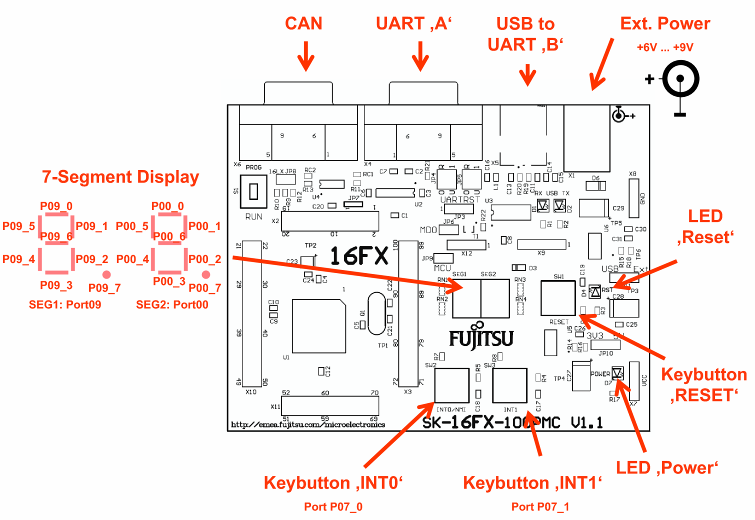
\includegraphics[width=0.7\textwidth]{starterkit}\end{center}

\subsection{p01\_7seg}
\label{exercise7Segment}

Implementiere ein Programm, das die Zahlen 0 bis 99 auf der Sieben-Segment-Anzeigen ausgibt.
Nach jeder Ausgabe einer Zahl soll eine Pause eingelegt werden.
Hinweise:\begin{itemize}
\item 
Für die Ausgabe der Zahlen 0 bis 9 steht Ihnen ein Array \textbf{\emph{DEC7SEG}} zur Verfügung, welches die benötigten Werte für die Ports für die jeweiligen Ziffern enthält.

\item 
Die Pause kann durch eine Schleife produziert werden, die in jedem Zyklus den Befehl \texttt{\_\_wait\_nop()} aufruft.
Eine Konstante \textbf{\emph{DELAY}} steht dir zur Verfügung für die Anzahl der Schleifendurchläufe.
Achte insbesondere darauf, dass du für die Schleifenzählervariable den Datentyp \emph{long} verwendst:
\begin{lstlisting}
int main(void) {
    long d;
    // ...
    for (d = 0; d < DELAY; ++d) {
        __wait_nop();
    }
}
\end{lstlisting}

\item
Die beiden Anzeigen sind an den \textbf{Ports 09} und \textbf{00} angeschlossen.
Die Ansteuerung erfolgt logisch invertiert, das bedeutet, wenn ein Ausgang für ein Segment logisch 0 ist, leuchtet dieses, bei 1 ist es aus.

\item
Beispiel: ein \glqq{}E\grqq{} kann durch das Setzen der Pins 0, 3, 4, 5 und 6 auf low gezeichnet werden.\footnote{
	Im Internet gibt es zahlreiche (Online-)Tools zum Umrechnen, z.B. 
	\url{http://binaer-dezimal-hexadezimal-umrechner.miniwebapps.de/}
}

\quad Binär: 10000110

\quad Hexadezimal: 0x86

\item
Es kann sinnvoll sein, deine Anzeige für hexadezimale Zeichen zu erweitern.
Ergänze dazu das Array \emph{DEC7SEG}, sodass die Zahlen 10 bis 15 als \texttt{A},\dots,\texttt{F} dargestellt werden können.

\end{itemize}
\begin{center}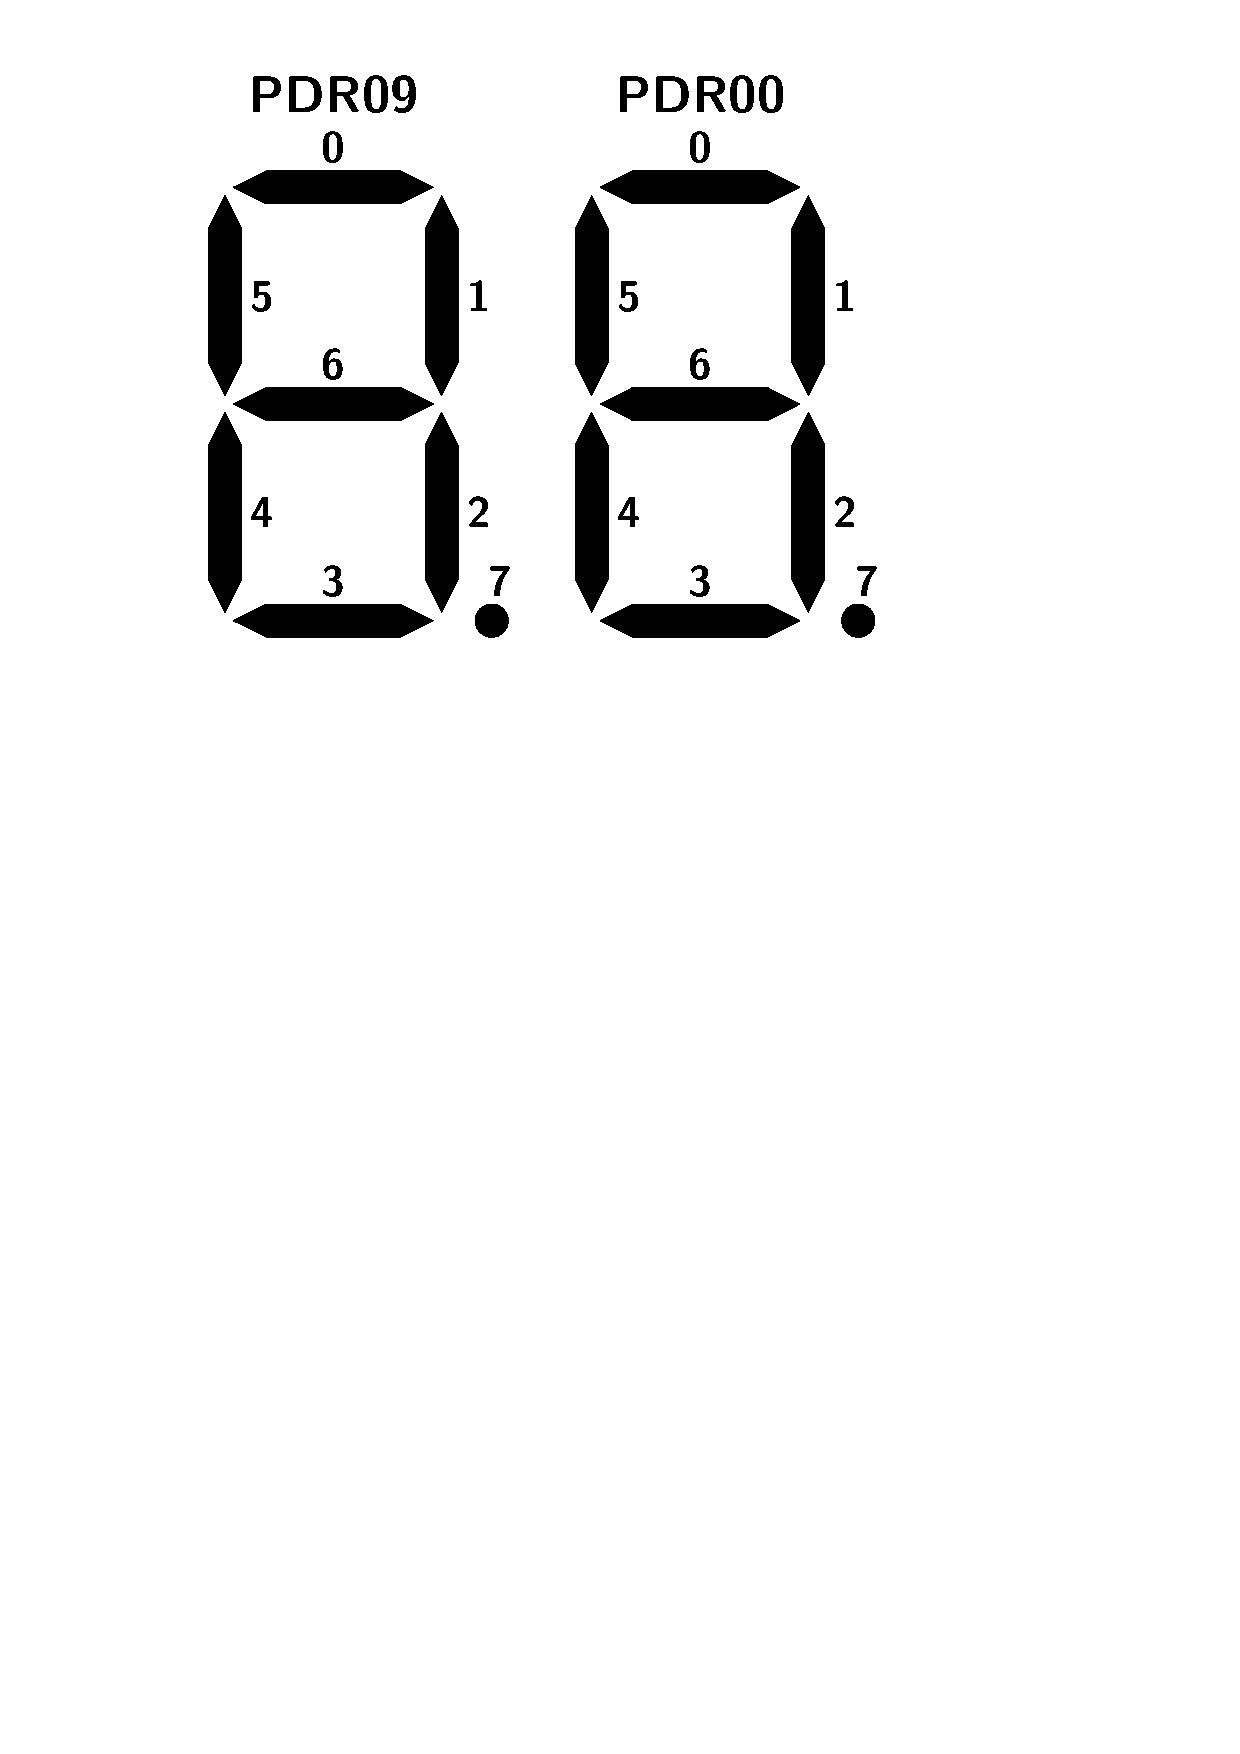
\includegraphics[width=0.3\textwidth]{7seg}\end{center}

\subsection{p02\_buttons}
Erstelle einen Counter.
Das Programm soll zu Beginn den Wert 00 anzeigen.
Bei Druck auf die rechte Taste soll der Wert erhöht, bei Druck auf die linke Taste verringert werden.
Wird 99 angezeigt und die rechte Taste gedrückt, soll der Counter auf 00 gesetzt werden.
Umgekehrt gilt:
Falls der Counter 00 anzeigt und die linke Taste gedrückt wird, soll er auf 99 umspringen.

Hinweise:\begin{itemize}
\item
Ein Button ist üblicherweise für mehrere tausend CPU-Zyklen gedrückt!

\item
Ein Tastendruck ist durch den Übergang von \emph{high} auf \emph{low} definiert.
Da in jedem Zyklus nur der aktuelle Wert abgefragt werden kann, musst du den aktuellen Wert mit einem gespeicherten Wert aus dem vorigen Durchlauf vergleichen.

\item
Der linke Taster ist an Port 07 Pin 0, der rechte an Port 7 Pin 1 angeschlossen.
Bei gedrücktem Taster liegt ein Low-Pegel am Eingang, sonst ein High-Pegel.
Du kannst den Zustand eines Pins wie folgt abfragen:
\begin{lstlisting}
char stateOfLeftButton = PDR07_P0; 
char stateOfRightButton = PDR07_P1;
\end{lstlisting}

\item
Die Moduloberechnung von negativen Zahlen kann problematisch werden.
Hier hilft es, wenn du vor der Modulooperation den Divisor hinzuaddierst.
Beispiel:
\begin{lstlisting}
int value = (value + 42) % 42;
\end{lstlisting}

\end{itemize}

\subsection{p03\_util}
\label{exercise7SegmentUtil}
Wie in \ref{exercise7Segment} sollen hier die Zahlen 0 bis 99 ausgegeben werden, jedoch unter Verwendung von eigens dafür geschriebenen Hilfsfunktionen:
\begin{lstlisting}
void wait(long w)          // wait for w cycles
void setLeft7Seg(int i)    // set left display to the given number i (if i is between 0 and 9)
void setRight7Seg(int i)   // set right display to the given number i (if i is between 0 and 9)
void set7Seg(int i)        // set the seven-segment display to the given number in the range of 0 to 99
\end{lstlisting}

\subsection{p04\_adc}
Schreibe ein Programm, das den Spannungswert von \emph{AN1} (linker Schieberegler) auf der linken Sieben-Segment-Anzeige und den Spannungswert von \emph{AN2} (rechter Schieberegler) auf der recht Sieben-Segment-Anzeige ausgibt.
Skaliere dazu den resultierenden Wertebereich (0 bis 255) auf 0 bis 9.\\

Verwende zur Initialisierung des A/D-Wandlers folgenden Code:
\begin{lstlisting}
// Start of function.
unsigned char result;

// Initialisation
ADCS_MD   = 3;		// ADC Stop Mode
ADCS_S10  = 1;		// 8 Bit Precision
ADER0_ADE1 = 1;	    // Activate analog inputs AN1 + AN2
ADER0_ADE2 = 1;     //  (ADER0: Inputs AN0 to AN7)
\end{lstlisting}
Anschließend kannst du mit folgendem Code (hier für den Kanal 1) eine A/D-Wandlung vornehmen:
\begin{lstlisting}
ADSR = 0x6C00 + (3 << 5) + 3;	      // Start and end channel is 1

ADCS_STRT = 1;				// Start A/D conversion
while (ADCS_INT == 0) { }	// Wait for A/D conversion to finish
result = ADCRL;			// store result (1 Byte)
ADCS_INT = 0;				// Set bit to 0 for next conversion
\end{lstlisting}

Hinweise:
\begin{itemize}
\item 
Einige Funktionen aus \ref{exercise7SegmentUtil} kannst du hier einsetzen.

\item 
Achte auf die richtige Initialisierung von \textit{ADER0}.

\item Der Wert für \textit{ADSR} besteht aus 16 Bits (0110 11xx xxxy yyyy\textsubscript{b}), wobei xxxxx für den Startkanal der Konvertierung und yyyyy für den Endkanal steht. Für unsere Zwecke nehmen diese beiden 5\,Bit Blöcke immer entweder 00001 (AN1) oder 00010 (AN2) an.
Daher sieht die Initialisierung von ADSR etwas kryptisch aus:
\begin{verbatim}
// Start and end channel is 3
ADSR = 0x6C00 + (3 << 5) + 3;
\end{verbatim}

\item
Lies die beiden Werte nacheinander aus, verwende also immer die gleiche Zahl für Start- und Endkanal während einer Konvertierung.

\end{itemize}

\subsection{p05\_lcdbasics}
Ziel dieser Aufgabe ist es, die linke Seite des Displays anzusteuern und alle Zellen mit dem Wert aa\textsubscript{h} (10101010\textsubscript{b}) zu belegen.

Hinweise:
\begin{itemize}
\item
Für diese Aufgabe benötigst du die Dokumentation des Displays (\textit{<SVN>/Doku/Display\_AV128641YFBY-WSV.pdf}), dort insbesondere den Abschnitt mit den Befehlen: Setzen der x- und y-Adresse, Einschalten des Displays, Senden von Daten.

\item
Achte darauf, nach jedem Befehl (Daten oder Instruktion) das Enable-Signal an das Display zu senden.
Es empfiehlt sich, eine Funktion \textit{void lcd\_sendEnable(void)} zu implementieren, die den Enable-Pin auf 1 setzt, kurz wartet und dann wieder auf 0 setzt und erneut kurz wartet.
Verwende als Warteintervall die Konstante \emph{LCD\_T}.
Denke daran, das Enable-Pin zu Beginn des Programms mit 0 zu initialisieren.

\item
Das Display ist logisch aufgeteilt in zwei Hälften zu je 64 x 64 Pixel (siehe untenstehende Grafik).
Welche Hälfte einen Befehl verarbeiten soll wird ausgewählt, in dem deren Chip-Select-Signal \emph{CS1} bzw. \emph{CS2} auf 1 gesetzt wird, das andere auf 0.

\item
Die Ansteuerung erfolgt über Pins mit festgelegten Funktionen. Zur Vereinfachung wurden bereits im Projekt für diese Aufgabe Definitionen vorgegeben, so dass die Pins über einfache Namen angesteuert werden können. Die Namen entsprechen den Pins, wie sie im Datenblatt ab Seite 10 zu finden sind.

\begin{center}
\begin{tabular}{l|l|l}
	\toprule
\textbf{Name} & \textbf{Funktion} & \textbf{Pin/Port} \\ 
 \midrule
LCD\_PORT\_DB & Datenbus (DB0 - DB7) & P01 \\ 
LCD\_PIN\_DI & Data (1) / Instruction (0) & P02\_0 \\ 
LCD\_PIN\_RW & Read (1) / Write (0) & P02\_1 \\ 
LCD\_PIN\_E & Enable & P02\_2 \\ 
LCD\_PIN\_CS1 & Linker Chip (1 = aktiv) & P02\_3 \\ 
LCD\_PIN\_CS2 & Rechter Chip (1 = aktiv) & P02\_4 \\ 
LCD\_PIN\_RESET & Reset-Signal (0 = aktiv) & P02\_5 \\ 
\bottomrule
\end{tabular}
\end{center}

\item
Grundsätzliches Prinzip zum Senden von Befehlen:
\begin{enumerate}
	\item
	Daten am Datenbus bereitstellen: PORT\_DB, PIN\_DI, PIN\_RW wie gewünscht setzen, ein Chip-Select (PIN\_CS1 oder PIN\_CS2) aktivieren
	
	\item
	Enable-Signal schicken (z.B. \textit{void lcd\_sendEnable(void)})
\end{enumerate}
Beachte: Das Reset-Signal muss immer 1 (deaktiviert) sein.

\item Vorgehen zum Schreiben von Bilddaten:
\begin{enumerate}
	\item Setzen der x-Adresse (Zeilenblock)
	\item Setzen der y-Adresse (Spalte)
	\item Senden von 8 Bit Daten (eine \glqq{}Zelle\grqq{} von 8 Pixeln Höhe)
\end{enumerate}
Vereinfachung: Der \textit{x}-Zähler wird nach dem Senden von Daten im Display automatisch hochgezählt.
Somit kann \textit{y} zu Beginn jeder Zeile auf 0 gesetzt werden und muss danach für den Rest der Zeile nicht mehr manuell gesetzt werden.

\begin{center}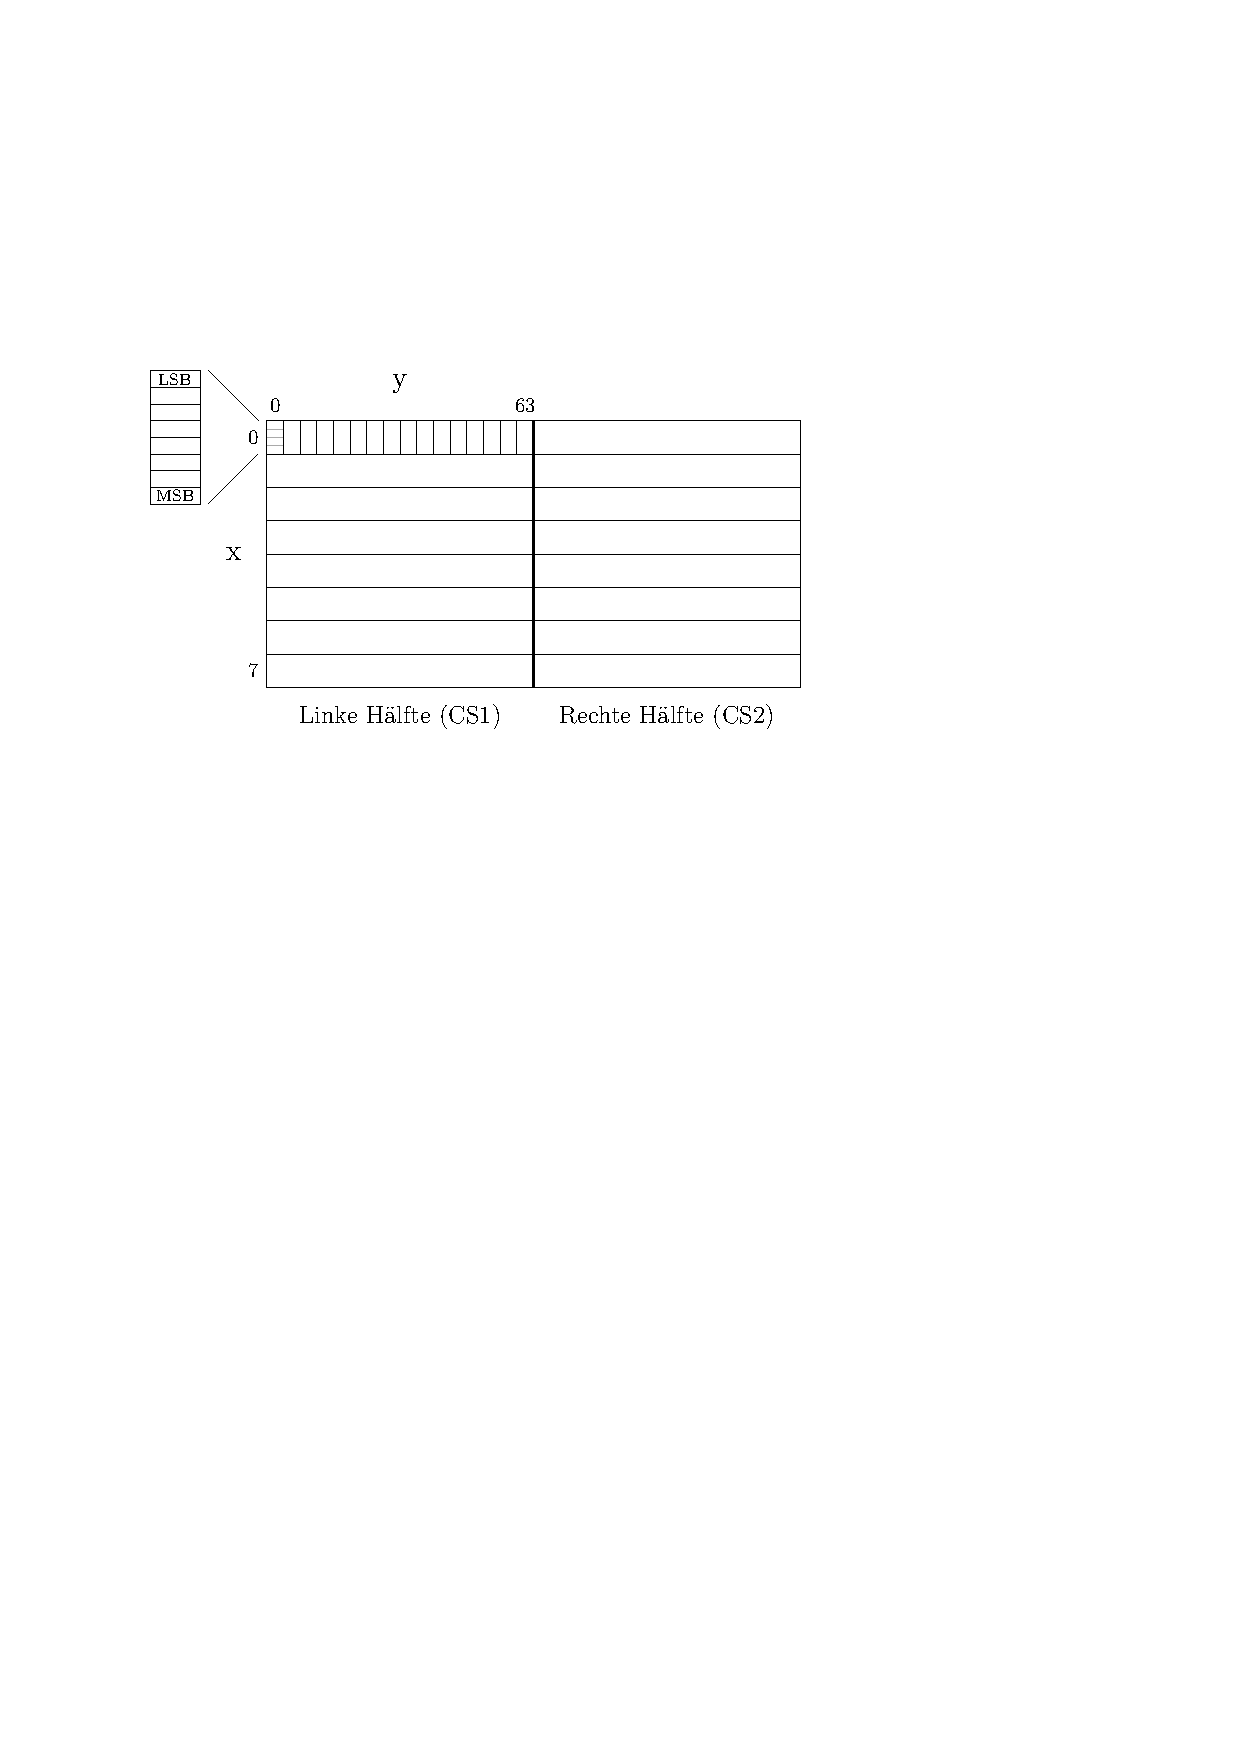
\includegraphics[width=0.6\textwidth]{display_aufbau}\end{center}


\end{itemize}

\subsection{p06\_lcd}
Nun soll das Display wie ein Bildschirm angesteuert werden können. Es gibt einen Buffer \textit{lcd\_buffer}, auf dem Pixeloperationen durchgeführt werden sollen. 
Schreibe folgende Funktionen:
\begin{lstlisting}
void lcd_clear()                             // Clear buffer (set all slots to 0)
void lcd_drawPixel(int x, int y, int black)  // Sets a pixel at (x,y) if black == 1
                                             // Clears a pixel at (x,y) if black == 0
                                             // Ignore if x,y, or black is invalid
void lcd_flush()                             // Show buffer on display
\end{lstlisting}
Hinweise:
\begin{itemize}
\item 
Ein Testprogramm steht bereits zur Verfügung, welches ein Schachbrettmuster auf dem Display ausgibt -- wenn deine Funktionen komplett und korrekt implementiert sind.

\item
Achte auch hier darauf, dass das Display zunächst per Befehl eingeschaltet werden muss.

\item
Für die Funktion \textit{lcd\_drawPixel} werden Bitoperationen benötigt. Eine Skizze kann hier sinnvoll sein, um sich vorzustellen, wie die Bitoperationen arbeiten.
\end{itemize}


\end{document}
